\part{Reference}

\titleformat{\chapter}[display]{\Huge\bf}{}{0mm}{\centering}[]
\titlespacing{\chapter}{0mm}{0mm}{5mm}

\chapter{Regiments}

\titleformat{\subsection}[display]{\small\bf}{}{0mm}{}[]

\subsection*{Royal Horse Guards (RHG)}

\begin{itemize}
\item Raised in 1650
\item Amalgamated with 1D to form RHG/D in 1969
\end{itemize}

\subsection*{Life Guards (LG)}

\begin{itemize}
\item Raised in 1660
\item Part of the Household Cavalry Regiment from 1992
\end{itemize}

\subsection*{1\st (Royal) Dragoons (1D)}

\begin{itemize}
\item Raised in 1661
\item Amalgamated with RHG to form RHG/D in 1969
\end{itemize}

\subsection*{1\st (King's) Dragoon Guards (1DG)}

\begin{itemize}
\item Raise in 1685
\item Amalgamated with 2DG to form QDG in 1959
\end{itemize}

\subsection*{3rd (Prince of Wales') Dragoon Guards (3DG)}

\begin{itemize}
\item Raised in 1685
\item Amalgamated with 6D to form 3C in 1922
\end{itemize}

\subsection*{4\nth (Royal Irish) Dragoon Guards (4DG)}

\begin{itemize}
\item Raised in 1685
\item Amalgamated with 7DG, to form the 4/7DG in 1922
\end{itemize}

\subsection*{Carabiniers (6\nth Dragoon Guards) (6DG)}

\begin{itemize}
\item Raised in 1685
\item Amalgamated with 5DG to form 3C in 1922
\end{itemize}

\subsection*{7\nth (The Princess Royal's) Dragoon Guards (7DG)}

\begin{itemize}
\item Raised in 1688
\item Amalgamated with 4DG, to form 4/7DG in 1922
\end{itemize}

\subsection*{5\nth Royal Irish Lancers (5L)}

\begin{itemize}
\item Raised in 1689
\item Amalgamated with 16L to become the 16/5L in 1922
\end{itemize}

\subsection*{6\nth (Inniskilling) Dragoons (6D)}

\begin{itemize}
\item Raised in 1689
\item Amalgamated with 5D to form 5 INNIS DG in 1922
\end{itemize}

\subsection*{9\nth (Queen's Royal) Lancers (9L)}

\begin{itemize}
\item Raised in 1715
\item Amalgamated with 12L to form 9/12L in 1960
\end{itemize}

\subsection*{11\nth (Prince Albert's Own) Hussars (11H)}

\begin{itemize}
\item Raised in 1715
\item Amalgamated with 10H to form RH in 1969
\end{itemize}

\subsection*{15\nth (The King's) Hussars (15H)}

\begin{itemize}
\item Raised in 1759
\item Amalgamated with 19H to form 15/19H in 1922
\end{itemize}

\subsection*{16\nth Lancers (16L)}

\begin{itemize}
\item Raised in 1759
\item Amalgamated with 5L to form 16/5L in 1922
\end{itemize}

\subsection*{17\nth (Duke of Cambridge's Own) Lancers (17L)}

\begin{itemize}
\item Raised in 1759
\item Amalgamated with 21L to form 17/21L in 1922
\end{itemize}

\subsection*{20\nth Hussars (20H)}

\begin{itemize}
\item Raised in 1858
\item Amalgamated with 14H to form 14/20H in 1922
\end{itemize}

\subsection*{21\st (Empress of India's) Lancers (21L)}

\begin{itemize}
\item Raised in 1858
\item Amalgamated with 17L to form 17/21L in 1922
\end{itemize}

\subsection*{3rd Carabiniers (Prince of Wales's Dragoon Guards) (3C)}

\begin{itemize}
\item Amalgamated from 3DG and 6DG in 1922
\item Amalgamated with 2D to form SCOTS DG in 1971
\end{itemize}

\subsection*{4\th/7\nth Royal Dragoon Guards (4/7DG)}

\begin{itemize}
\item Amalgamated from 4DG and 7GD in 1922
\item Amalgamated with 5 INNIS DG to form RDG in 1992
\end{itemize}

\subsection*{5\nth Royal Inniskilling Dragoon Guards (5 INNIS DG)}

\begin{itemize}
\item Amalgamated from 5D and the 6D in 1922
\item Amalgamated with 4/7 DG to form RDG in 1992
\end{itemize}

\subsection*{13\th/18\nth Royal Hussars (Queen Mary's Own) (13/18 RH)}

\begin{itemize}
\item Amalgamated from 13H and 18H in 1922
\item Amalgamated with 15/19H to form LD in 1992
\end{itemize}

\subsection*{14\th/20\nth King's Hussars (14/20H)}

\begin{itemize}
\item Amalgamated from 14H and 20H in 1922
\item Amalgamated with the RH to form KRH in 1992
\end{itemize}

\subsection*{15\th/19\nth The King's Royal Hussars (15/19H)}

\begin{itemize}
\item Amalgamated from 15H and 19H in 1922
\item Amalgamated with 13/18 RH to form LD in 1992
\end{itemize}

\subsection*{16\th/5\nth The Queen's Royal Lancers (16/5L)}

\begin{itemize}
\item Amalgamated from 16L and 5L in 1922
\item Amalgamated with 17/21L to form QRL in 1993
\end{itemize}

\subsection*{17\th/21\st Lancers (17/21L)}

\begin{itemize}
\item Amalgamated from 17L and 21L in 1922
\item Amalgamated with 16/5L to form QRL in 1993
\end{itemize}

\subsection*{Queen's Own Hussars (QOH)}

\begin{itemize}
\item Amalgamated from 3H and 7H in 1958
\item Amalgamated with QRIH to form QRH in 1993
\end{itemize}

\subsection*{Queen's Own Royal Irish Hussars (QRIH)}

\begin{itemize}
\item Amalgamated from 4H and 8H in 1958
\item Amalgamated with QOH to form QRH in 1993
\end{itemize}

\subsection*{1\st The Queen's Dragoon Guards (QDG)}

\begin{itemize}
\item Amalgamated from KDG and 2DG in 1959
\end{itemize}

\subsection*{9\th/12\nth Royal Lancers (9/12L)}

\begin{itemize}
\item Amalgamated from 9L and 12L in 1960
\item Amalgamated into RL in 2015
\end{itemize}

\subsection*{Blues and Royals (Royal Horse Guards and 1\st Dragoons) (RHG/D)}

\begin{itemize}
\item Amalgamated from RHG and RD in 1969
\item Part of the Household Cavalry Regiment from 1992
\end{itemize}

\subsection*{The Royal Hussars (Prince of Wales's Own) (RH)}

\begin{itemize}
\item Formed from 10H and 11H in 1969
\item Amalgamated into KRH in 1992
\end{itemize}

\subsection*{Royal Scots Dragoon Guards (Carabiniers and Greys) (SCOTS DG)}

\begin{itemize}
\item Amalgamated from 3C and 2D in 1971
\end{itemize}

\subsection*{Household Cavalry Regiment (HCR)}

\begin{itemize}
\item Encompasses LG and RHG/D from 1992
\end{itemize}

\subsection*{King's Royal Hussars (KRH)}

\begin{itemize}
\item Amalgamated from RH and 14/20H in 1922
\end{itemize}

\subsection*{Light Dragoons (LD)}

\begin{itemize}
\item Amalgamated from 13/18 RH and 15/19 KRH in 1992
\end{itemize}

\subsection*{Royal Dragoon Guards (RDG)}

\begin{itemize}
\item Amalgamated from 4/7 DG and 5 INNIS DG in 1992
\end{itemize}

\subsection*{Queen's Royal Hussars (QRH)}

\begin{itemize}
\item Amalgamated from QOH and QRIH in 1993
\end{itemize}

\subsection*{Queen's Royal Lancers (QRL)}

\begin{itemize}
\item Amalgamated from 16/5L and 17/21L in 1993
\item Amalgamated with 9/12L to form RL in 2015
\end{itemize}

\subsection*{Royal Lancers (RL)}

\begin{itemize}
\item Amalgamated from 9/12L and QRL in 2015
\end{itemize}

\begin{figure}[h]
  \centering
  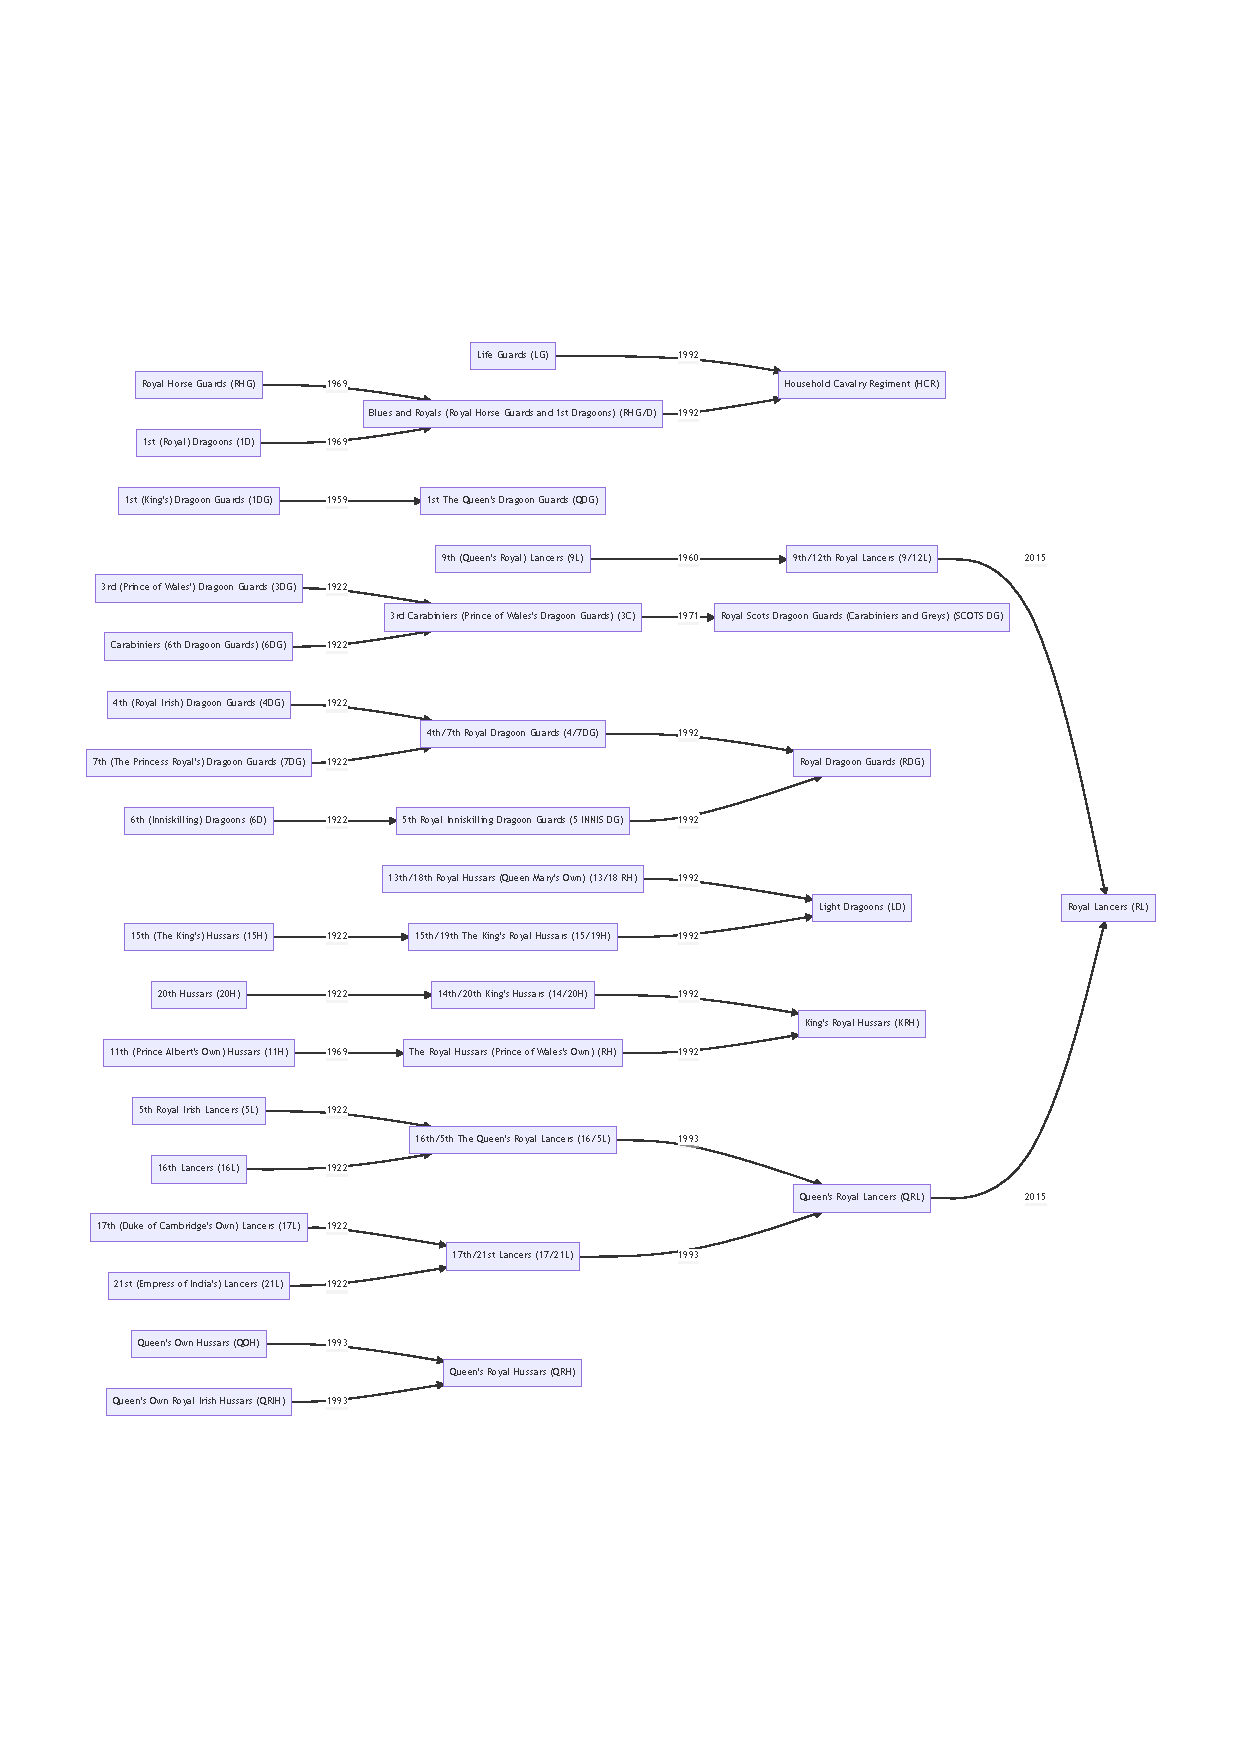
\includegraphics[width=1\textwidth]{reference/regiments.pdf}
\end{figure}
